
\documentclass[aspectratio=169]{beamer}
\usepackage{tikz}
\usetikzlibrary{shadows,shapes.geometric,positioning,arrows,shapes.misc,shadings}

\tikzset{diagonal fill/.style 2 args={fill=#2, path picture={
			\fill[#1, sharp corners] (path picture bounding box.south west) -|
			(path picture bounding box.north east) -- cycle;}},
	Lemma/.style={rectangle, draw, rounded corners} , 
	Definition/.style={chamfered rectangle, draw} , 
	File/.style={rectangle,draw,text width=7em},
	FSM/.style={fill=blue!20},
	FSM_Product/.style={fill=yellow!20},
	ATC/.style={fill=cyan!20},
	ASC_LB/.style={fill=orange!20},
	ASC_Suite/.style={fill=lime!20},
	ASC_Sufficiency/.style={fill=lightgray!20},
	ASC_Hoare/.style={fill=magenta!20},
	line/.style = {lightgray,draw, -latex'},
	lineNew/.style = {red, thick, draw, -latex'},
           New/.style = {red, thick, text=black}
}


\begin{document}
\beamertemplatenavigationsymbolsempty

\author{Robert Sachtleben}
\title{Proof Overview}
\subtitle{concerning the correctness of the refined adaptive state counting algorithm}
\date{\today}

\maketitle


\begin{frame}%{Overview of the correctness proof}


\begin{figure}
\begin{tikzpicture}[node distance = 1cm, auto, every node/.style={scale=0.55, text badly centered, minimum height=2.5em, align=center}]

\onslide<+-> {
        \node [Definition,FSM, anchor=north]                            (FSMs)          {FSMs $M,M'$  \\ {\tiny \texttt{record FSM}}};
        \node [Definition,FSM, right=0.8cm of FSMs]                            (V)          {$detSC(V)$ \\ {\tiny \texttt{is\_det\_state\_cover}}};
}
 
\onslide<+->{
        \node [Lemma,FSM_Product, below=1 cm of FSMs.west, anchor=west]                        (mFV_ex)         {$\neg M' \preceq M \longrightarrow \exists xs . mFV(xs)$ \\ {\tiny \texttt{minimal\_sequence\_to\_failure\_extending\_det\_state\_cover\_ob}} };
        \path [line] (FSMs)         --                              (mFV_ex); 
        \path [line] (V)         --                              (mFV_ex);   
}
\onslide<+->{
        \node [Definition,ATC, right=0.8cm of V]                            (ATC)          {ATCs \\ {\tiny \texttt{datatype ATC}}};
}
\onslide<+->{
        \node [Definition,ASC_LB, right=0.8cm of ATC]                            (LB)          {fun $LB$ \\ {\tiny \texttt{fun LB}}};
        \node [Definition,ASC_LB, right=0.8cm of LB]                            (SizeAssm)          {$|M'| \leq m$ \\ {\tiny \texttt{fault\_domain}}};
}
\onslide<+->{
        \node [Lemma,diagonal fill={orange!20}{yellow!20},right =0.5cm of mFV_ex]                            (minLB)          {$noRep(xs) \longrightarrow |M'| \geq LB (xs)$ \\ {\tiny \texttt{LB\_count}}};
        \path [line] (LB)         --                              (minLB);   
        \path [line] (ATC)         --                              (minLB);  
}
\onslide<+->{
        \node [Definition,ASC_Suite, right=0.8cm of SizeAssm.east, anchor=west]                            (TS)          {test suite $TS$ \\ {\tiny \textit{fun TS, final\_iteration\_ex}}};
}
\onslide<+->{
%        \node [Lemma,ASC_Suite, below=2cm of TS.east, anchor=east,label={[align=left,shift={(3.5,-0.3)}]*}]                            (elemTS)          {$in(xs) \not\in TS \longrightarrow LB(xs) > m \vee M'\not\preceq_{TS}M$ \\ {\tiny \texttt{TS\_non\_containment\_causes\_final}}};
        \node [Lemma,ASC_Suite, below=2cm of TS.east, anchor=east]                            (elemTS)          {$in(xs) \not\in TS \longrightarrow LB(xs) > m \vee M'\not\preceq_{TS}M$ \\ {\tiny \texttt{TS\_non\_containment\_causes\_final}}};
        \path [line] (TS)         --                              (elemTS);   
}


\onslide<+->{
        \node [Lemma,ASC_Sufficiency, below=2cm of V.west, anchor=west]                            (noRep)          {$mFV(xs) \longrightarrow noRep(xs)$\\ {\tiny \textit{mstfe\_distinct\_Rep\_Pre}, \textit{mstfe\_distinct\_Rep\_Cov}}};
        \path [line] (mFV_ex) -- (noRep); 
}

\onslide<+->{
        \node [Lemma,ASC_Sufficiency, below=1cm of elemTS.east, anchor=east]                                                       (elemTSmin)          {$M'\preceq_{TS}M \longrightarrow \exists xs . mFV(xs) \wedge in(xs) \notin TS \longrightarrow |M'| > m$ \\ {\tiny proof idea of \texttt{asc\_sufficiency}}};
        \path [line] (elemTS)         --                              (elemTSmin);   
        \path [line] (minLB)         edge[bend right=20]                              (elemTSmin);   
        \path [line] (noRep)     --                                (elemTSmin);
}

\onslide<+->{
        \node [Lemma,ASC_Sufficiency, below=3cm of mFV_ex.west, anchor=west]                            (9)          {$M'\preceq_{TS}M \longrightarrow M' \preceq M$ \\ {\tiny \texttt{asc\_sufficiency}}};
        \path [line] (mFV_ex) -- (9);   
        \path [line] (elemTSmin)  edge[bend left=7]  (9); 
        \path [line] (SizeAssm)      edge[bend left=18]                                (9);
}

\onslide<+->{
        \node [Lemma,ASC_Sufficiency, below=1cm of 9.north]                            (10)          {$M' \preceq M \longleftrightarrow M' \preceq_{TS} M$ \\ {\tiny \texttt{asc\_main\_theorem}}};
        \path [line] (9) -- (10);
}
\onslide<+->{
        \node [Definition,ASC_Hoare, below=2cm of elemTS.east, anchor=east]                            (11)          {algorithm in WHILE language};
}
\onslide<+->{
        \node [Lemma,ASC_Hoare, below=1cm of 11.east, anchor=east]                            (12)          {algorithm applies $TS$ until failure \\ {\tiny loop invariant of \texttt{refined\_adaptive\_state\_counting\_correctness}}};
        \path [line] (11) -- (12);
}
\onslide<14-15>{
        \node [Lemma,ASC_Hoare, below=1cm of 10.west, anchor = west]                            (13)          {algorithm returns \texttt{true} if and only if $M' \preceq M$ \\ {\tiny post-condition of  \texttt{refined\_adaptive\_state\_counting\_correctness}}};
        \path [line] (10) -- (13);
        \path [line] (12) -- (13);
}

\only<2>{
        \path [lineNew] (FSMs) --                             (mFV_ex); 
        \path [lineNew] (V)         --                              (mFV_ex);   
}
\only<5>{
        \path [lineNew] (LB)         --                              (minLB);   
        \path [lineNew] (ATC)         --                              (minLB);  
}
\only<7>{
        \path [lineNew] (TS)         --                              (elemTS);   
}
\only<8>{
        \path [lineNew] (mFV_ex) -- (noRep); 
}
\only<9>{
        \path [lineNew] (elemTS)         --                              (elemTSmin);   
        \path [lineNew] (minLB)         edge[bend right=20]                              (elemTSmin);   
        \path [lineNew] (noRep)     --                                (elemTSmin);
}
\only<10>{
        \path [lineNew] (mFV_ex) -- (9);   
        \path [lineNew] (elemTSmin)  edge[bend left=7]  (9); 
        \path [lineNew] (SizeAssm)      edge[bend left=18]                                (9);
}
\only<11>{
        \path [lineNew] (9) -- (10);
}
\only<13>{
        \path [lineNew] (11) -- (12);
}
\only<14>{
        \path [lineNew] (10) -- (13);
        \path [lineNew] (12) -- (13);
}


\end{tikzpicture}
\hspace{0.2cm}
\vrule{}
\hspace{0.2cm}
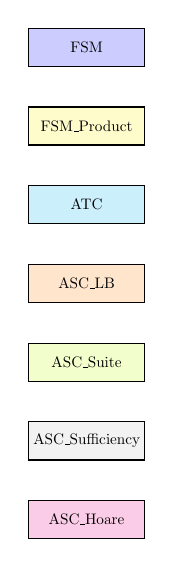
\begin{tikzpicture}[node distance = 1cm, auto, every node/.style={scale=0.55, text badly centered, minimum height=2.5em}]
        % Step 1
        \node [FSM,File]                            (FSM_File)          {FSM};
\onslide<2->{
        \node [FSM_Product,File, below=1cm of FSM_File.north]                        (FSM_Product_File)         {FSM\_Product};
}
\onslide<3->{
        \node [ATC,File, below=1cm of FSM_Product_File.north]                        (ATC_File)         {ATC};
}
\onslide<4->{
        \node [ASC_LB,File, below=1cm of ATC_File.north]                        (ASC_LB_File)         {ASC\_LB};
}
\onslide<6->{
        \node [ASC_Suite,File, below=1cm of ASC_LB_File.north]                        (ASC_Suite_File)         {ASC\_Suite};
}
\onslide<8->{
        \node [ASC_Sufficiency,File, below=1cm of ASC_Suite_File.north]                        (ASC_Sufficiency_File)         {ASC\_Sufficiency};
}
\onslide<12->{
        \node [ASC_Hoare,File, below=1cm of ASC_Sufficiency_File.north]                        (ASC_Hoare_File)         {ASC\_Hoare};
}

\end{tikzpicture}
\end{figure}

\hrule{}

\centering
    \scalebox{0.5}{\parbox{.9\textwidth}{%
    \begin{align*}
    \only<1>{detSC(V) &= \text{$V$ is a deterministic state cover of $M$}  \\}
    \onslide<2->{detSC(V) &= \text{$V$ is a deterministic state cover of $M$} & mFV(xs) &= \text{$xs$ is a minimal sequence to failure extending $V$} \\}
    \only<5-6>{noRep(xs) &= \text{$xs$ does not repeat any state of the product machine of $M$ and $M'$} \\ }
    \onslide<7->{noRep(xs) &= \text{$xs$ does not repeat any state of the product machine of $M$ and $M'$} \qquad & in(xs) &= \text{input portion of $xs$} \\}
    \end{align*}
    }}

%\footnotetext[1]<1->{det. SC = deterministic state cover of $M$}
%\footnotetext[2]<2->{mFV = minimal sequence to failure extending $V$}
%\footnotetext[3]<6->{in = input portion}
\end{frame}





\begin{frame}{Current state}
\begin{itemize}
	\item Correctness of the ASC-algorithm has been proven
	\begin{itemize}
		\item Further refinements proved necessary
		\item $>9k$ LoC
	\end{itemize}
  
    \item Completeness of testing by applying all sequences of length up to $m*n$ 
    \begin{itemize}
    	\item Currently only for observable FSMs
    \end{itemize}
\end{itemize}
\end{frame}

\begin{frame}{TODO}
\begin{itemize}
	\item Code cleanup \& documentation
	\begin{itemize}
		\item AFP style guidelines
	\end{itemize}
	\item Maybe: comparison between ASC and '$m*n$'-Suite
	\item Maybe: add results for non-observable FSMs
\end{itemize}
\end{frame}


\end{document}